% LSTM part of the team report. Numbers are from a single run (seed 42) on the team's fixed test split (299 responses).
\subsection{LSTM model and training}
\paragraph{Preprocessing.} Text is lowercased and split into tokens with a regular expression. Words (including contractions), punctuation marks and newlines are separate tokens, and markdown markers (bold \texttt{**}, header \texttt{\#}, code fences and numbered-list markers such as ``1.'') are kept as their own tokens because formatting may be a signal. Numbers are mapped to a single \texttt{<num>} token. The vocabulary (at most 30{,}000 tokens, minimum frequency 2) is built from the training split only. Responses are truncated to 512 tokens and prompts to 128 tokens; sequences are packed, so padding is never fed to the LSTM. We use the team's fixed splits (2400 train, 301 validation, 299 test) in which no prompt appears in more than one split.

\paragraph{Architecture.} Each token is mapped to a 128-dimensional embedding trained from scratch and passed through a one-layer bidirectional LSTM with 128 hidden units per direction. The hidden states are summarized in two ways: attention pooling (a learned weighted average over time steps) and max pooling over time. The two 256-dimensional vectors are concatenated and passed through dropout $0.4$, a linear layer to 256 units with ReLU, dropout $0.4$, and a linear layer with three logits (Claude, GPT, Gemini). For the input+output setting the prompt and response are joined as one sequence, \texttt{prompt <sep> response}, and read by the same LSTM. The output-only model has about 2.5 million trainable parameters.

\paragraph{Training.} AdamW with learning rate $2\times10^{-3}$, weight decay $10^{-4}$, batch size 32, at most 15 epochs, and gradient clipping at norm 1.0. The loss is unweighted cross-entropy (the classes are nearly balanced). The learning rate is halved when validation macro-F1 does not improve for one epoch. We stop when validation macro-F1 has not improved for 4 epochs and evaluate the best epoch on the test set once. Each setting was run once, with seed 42.

\subsection{LSTM results}
\begin{table}[h]
\centering
\begin{tabular}{lccc}
Setting & Accuracy & Macro-F1 & Chance accuracy\\\hline
Output only (RQ1) & $0.799$ & $0.790$ & $0.333$\\
Input only (RQ2) & $0.348$ & $0.345$ & $0.333$\\
Input + output (RQ2) & $0.793$ & $0.784$ & $0.333$\\\hline
\end{tabular}
\caption{LSTM test results, single run (seed 42).}
\end{table}

\begin{figure}[h]
\centering
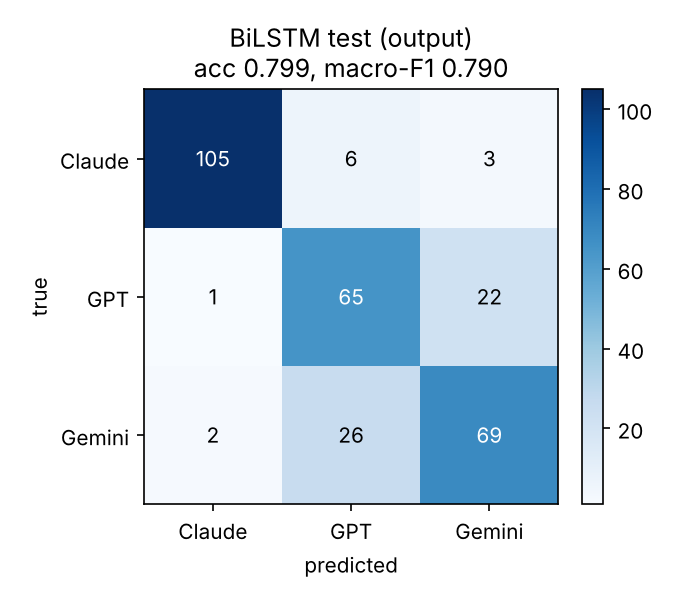
\includegraphics[width=0.4\textwidth]{results_lstm/lstm_output_confusion.png}
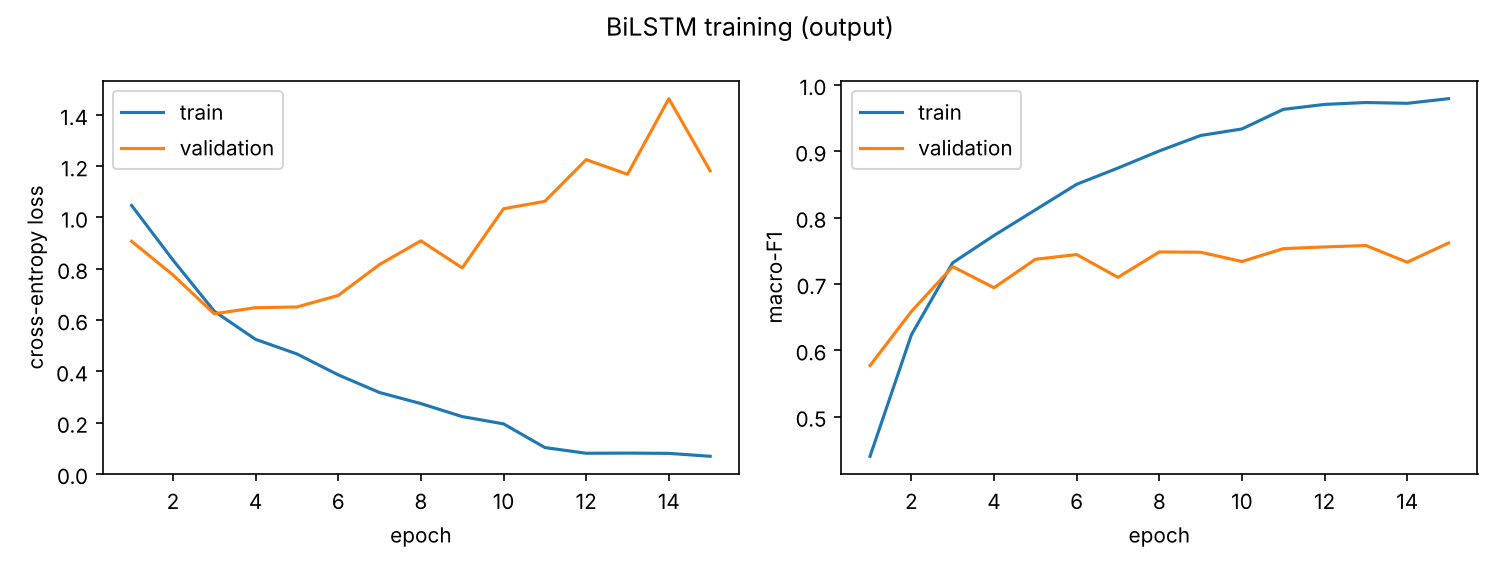
\includegraphics[width=0.58\textwidth]{results_lstm/lstm_output_curves.png}
\caption{Left: confusion matrix of the output-only LSTM on the test set. Right: training and validation loss and macro-F1 per epoch for the same model.}
\end{figure}

\paragraph{RQ1.} The LSTM identifies the LLM from the response alone with about 80\% accuracy, well above the 33\% chance level. Per-class F1 is $0.95$ for Claude, $0.72$ for Gemini and $0.70$ for GPT. Most errors are between GPT and Gemini (48 of the 60 errors), while Claude is rarely confused with either model (105 of 114 Claude responses are classified correctly).

\paragraph{RQ2.} The prompt alone gives close to chance accuracy ($0.348$), and adding the prompt to the response does not help ($0.793$ vs $0.799$, a difference of two test examples). The best input-only epoch was the first one, and its validation macro-F1 ($0.42$) did not carry over to the test set, which suggests the model found no stable signal in the prompts. This agrees with how the splits were built: each prompt is in a single split and the prompts come from a common pool of user questions. A small number of prompts were answered by two different families in the original battles (56 prompts, 116 responses in the training set), so the prompt cannot fully determine the label even in principle.

\paragraph{Comparison with the CNN.} The LSTM and the CNN reach almost the same performance. For output only the LSTM scores $0.799$ accuracy and $0.790$ macro-F1 against $0.803\pm0.008$ and $0.793\pm0.009$ for the CNN, and both models make the same kind of error (GPT vs Gemini). The LSTM is slightly better on Claude ($0.95$ vs $0.92$ F1) and slightly worse on GPT and Gemini, but these differences are a few test examples each. Since the LSTM reads the response in order and the CNN only sees local n-gram windows, the similar results suggest that local cues such as word choice, phrasing and formatting carry most of the signal.

\paragraph{Training behavior.} The output-only model overfits after the first few epochs: training macro-F1 reaches $0.98$ while validation loss rises from its minimum of $0.62$ at epoch 3 to $1.18$ at epoch 15. Validation macro-F1 still improves slowly over the same period (from $0.73$ to $0.76$), so early stopping on macro-F1 keeps the last epoch. The best epoch was the final allowed epoch, so a longer schedule might give a small further gain.

\paragraph{Caveats.} The test set has 299 examples, so one standard error of accuracy is about 2.3 points, larger than the differences between the LSTM settings and between the LSTM and the CNN. The LSTM results come from a single seed, while the CNN results are averaged over three, so the LSTM numbers have no error bars and run-to-run variation is not measured. The LSTM also uses longer inputs (512 vs 256 response tokens) and lowercased text, so the comparison with the CNN is between the two models as configured, not a controlled test of the architecture alone. Each ``family'' mixes several model versions from the Chatbot Arena data, and the three classes are balanced by construction (1000 each), which is not the natural distribution.
